\documentclass[11pt]{article}

% --- CONFIGURAÇÃO GEOMÉTRICA PARA SMARTPHONES (Proporção 9:16) ---
\usepackage[paperwidth=108mm, paperheight=192mm, margin=6mm]{geometry}

% --- PACOTES FUNDAMENTAIS ---
\usepackage[utf8]{inputenc}
\usepackage[T1]{fontenc}
\usepackage[sfdefault]{roboto} 
\usepackage[brazilian]{babel}
\usepackage{graphicx}
\usepackage{graphbox} 
\usepackage{xcolor}
\usepackage{fontawesome5}
\usepackage{caption}
\usepackage{parskip}
\usepackage{microtype}
\usepackage{tcolorbox}
\usepackage{tikz}

% --- PALETA DE CORES ---
\definecolor{NordBg}{HTML}{111418}
\definecolor{NordText}{HTML}{D8DEE9}
\definecolor{NordSky}{HTML}{5C87A6}       
\definecolor{AdguardGreen}{HTML}{28C86F}
\definecolor{BraveOrange}{HTML}{FF5722}
\definecolor{NordBlue}{HTML}{5E81AC}
\definecolor{NordPurple}{HTML}{B48EAD}
\definecolor{AccentYellow}{HTML}{F1C40F}  

% --- CORES DOS IPÊS ---
\definecolor{IpeAmarelo}{HTML}{F1C40F} 
\definecolor{IpeRosa}{HTML}{FF69B4}    
\definecolor{IpeBranco}{HTML}{FFFFFF}  
\definecolor{IpeRoxo}{HTML}{CD58C9}     

% --- CONFIGURAÇÃO DE LINKS ---
\usepackage[hidelinks]{hyperref}
\hypersetup{
    colorlinks=true,
    linkcolor=NordSky,
    urlcolor=AdguardGreen
}

% --- CONFIGURAÇÃO GLOBAL DE CORES ---
\pagecolor{NordBg}
\color{NordText}

% --- MACRO PARA OS PASSOS DIDÁTICOS ---
\newcommand{\passo}[3]{
    \vspace{2mm}
    \noindent \textcolor{#1}{\faMobile*}\textbf{\,\,\textcolor{#1}{Passo #2: }}{\small #3}\par
}

\begin{document}

% ================= PÁGINA 1: CAPA FULL BLEED =================
\newgeometry{margin=0pt}
\thispagestyle{empty}
\noindent
\begin{tikzpicture}[remember picture, overlay]
    \node[inner sep=0pt, anchor=center] at (current page.center) {%
        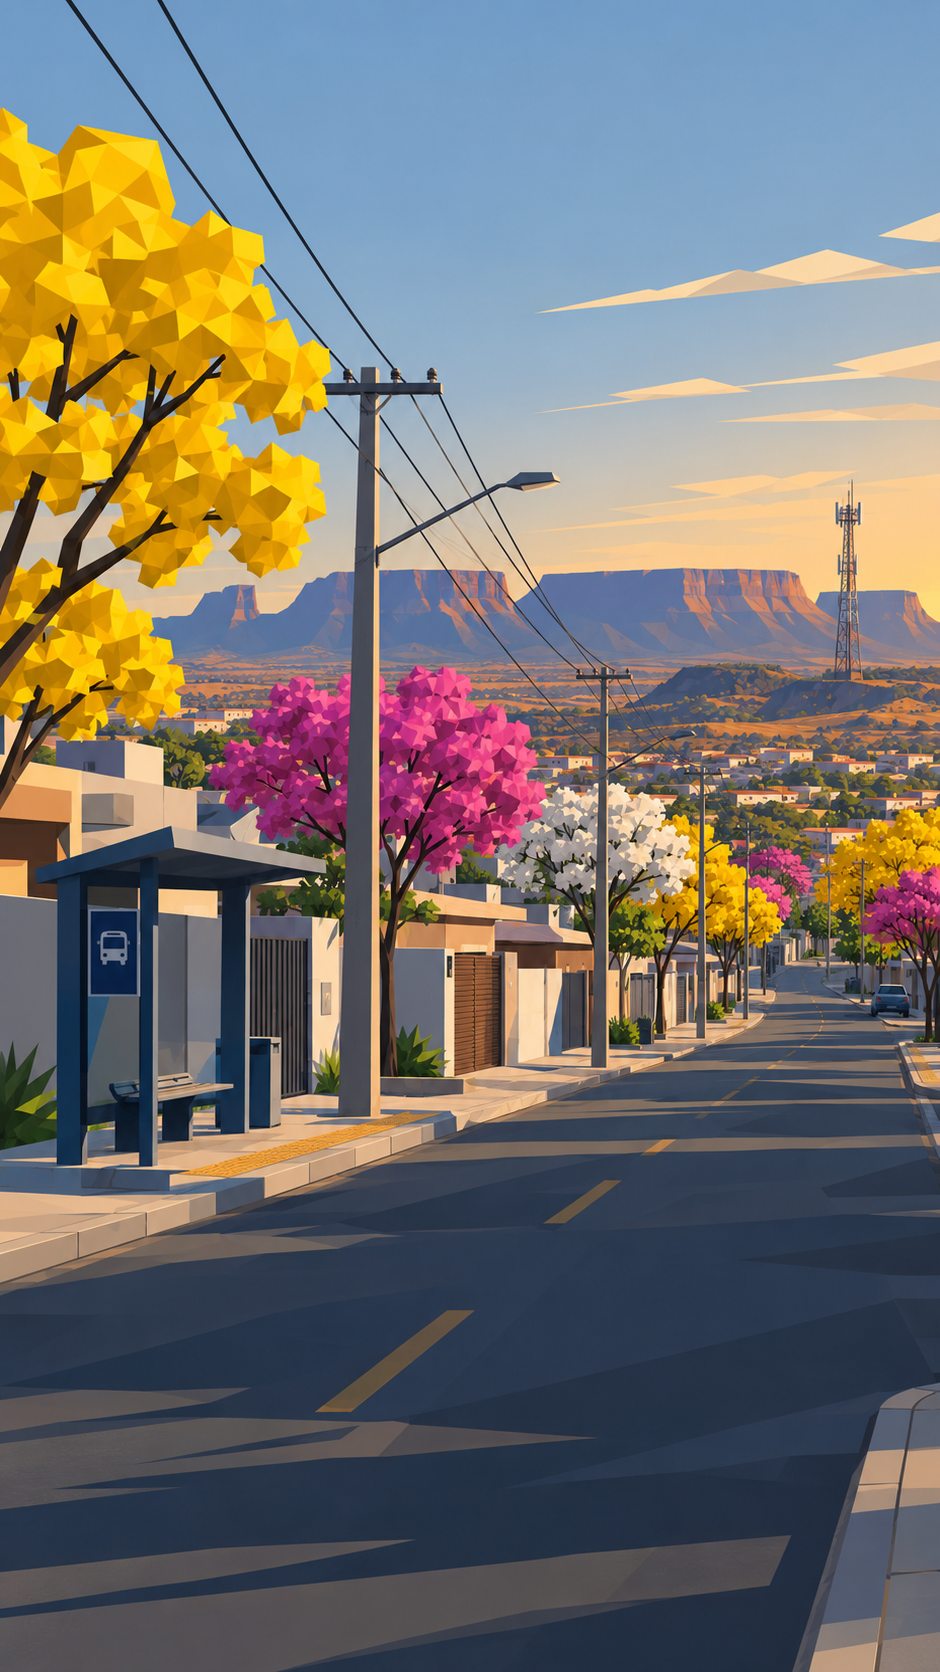
\includegraphics[width=\paperwidth, height=\paperheight]{../../assets/capa_guia_9_16.png}%
    };

    \node[
        anchor=north,
        yshift=-18mm,
        fill=NordBg,
        fill opacity=0.90,
        text opacity=1,
        draw=IpeAmarelo,
        line width=1.2pt,
        rounded corners=8pt,
        inner xsep=5mm,
        inner ysep=4mm,
        align=center
    ] at (current page.north) {
        {\footnotesize \textbf{\textcolor{IpeAmarelo}{\faLeaf \ SOBRIEDADE DIGITAL}}}\\[1.5mm]
        {\Large \textbf{\textcolor{IpeBranco}{Mini-Guia de Eficiência Energética Móvel}}}\\[1mm]
        {\small \textbf{\textcolor{IpeRosa}{Para Educadores e Comunidade Escolar}}}\\[2.5mm]
        {\tiny \textcolor{NordText!60}{Desenvolvido por: \textbf{\textcolor{IpeRoxo}{@naygno}}}}
    };

    \node[
        anchor=south,
        yshift=8mm,
        fill=NordBg,
        fill opacity=0.80,
        text opacity=1,
        draw=NordSky!50,
        line width=0.5pt,
        rounded corners=4pt,
        inner xsep=3mm,
        inner ysep=1.5mm
    ] at (current page.south) {
        \tiny \textcolor{IpeBranco!90}{Ciência da Computação \textbf{|} UFBRA}
    };
\end{tikzpicture}
\restoregeometry
\clearpage

% ================= PÁGINA 2: INTRODUÇÃO =================
\begin{center}
    \Large{\textbf{\textcolor{AccentYellow}{\faLeaf \ Sobriedade Digital}}}
    \vspace{1mm}
    \normalsize{\textcolor{NordSky}{\textbf{Guia de Eficiência Energética para Educadores}}}
\end{center}

\vspace{1mm}
\hrule
\vspace{4mm}

{\small \textbf{A Nuvem é Física (E ela consome água):} O ecossistema digital consome cerca de 10\% da eletricidade global. Cada requisição oculta e anúncio invasivo exige processamento ininterrupto em Data Centers resfriados por milhões de litros de água potável (métrica WUE).}

\vspace{3mm}

{\small \textbf{O Dreno de Bateria e Tail Energy:} Pesquisas canônicas (ACM EuroSys) comprovam que até 75\% da energia de apps gratuitos é consumida por rastreadores e telemetria de anúncios. Isso superaquece o SoC, degrada as baterias de lítio e força a substituição precoce do aparelho — alimentando as 62 milhões de toneladas anuais de lixo eletrônico.}

\vspace{3mm}

{\small Siga as etapas deste guia para estancar o processamento ocioso no seu smartphone. Utilize este material como recurso pedagógico alinhado aos \textbf{Temas Contemporâneos Transversais da BNCC} (Meio Ambiente e Tecnologia).}

\vfill
\begin{center}
    \tiny{\textcolor{NordText!50}{Projeto Multidisciplinar em Ciência da Computação | UFBRA}}
\end{center}

\newpage

% ================= PÁGINA 3: SEÇÃO 1 (DNS PRIVADO) =================
\large{\textbf{\textcolor{AdguardGreen}{1. Bloquear Rastreamento (DNS Privado)}}}
\normalsize

\passo{AdguardGreen}{1}{Abra as \textbf{Configurações} do celular e vá em \textbf{Rede e Internet} (ou Conexões).}
\passo{AdguardGreen}{2}{Toque em \textbf{DNS Privado} e selecione "Nome do host do provedor".}
\passo{AdguardGreen}{3}{Digite \texttt{family.adguard-dns.com} e salve. (Elimina anúncios na raiz da rede e corta requisições de fundo).}

\vspace{4mm}
\begin{minipage}[t]{0.48\textwidth}
    \centering
    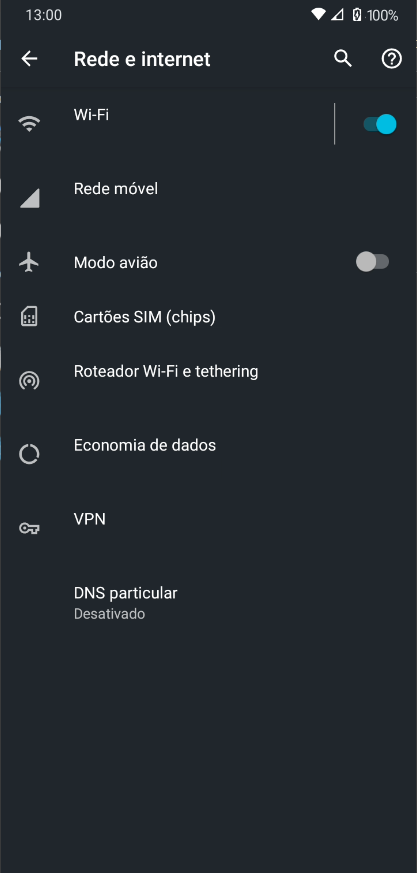
\includegraphics[align=c, width=\textwidth]{../../assets/screenshots/print_rede.png}
    \captionof*{figure}{\footnotesize \textcolor{NordText!80}{Rede e Internet}}
\end{minipage}
\hfill
\begin{minipage}[t]{0.48\textwidth}
    \centering
    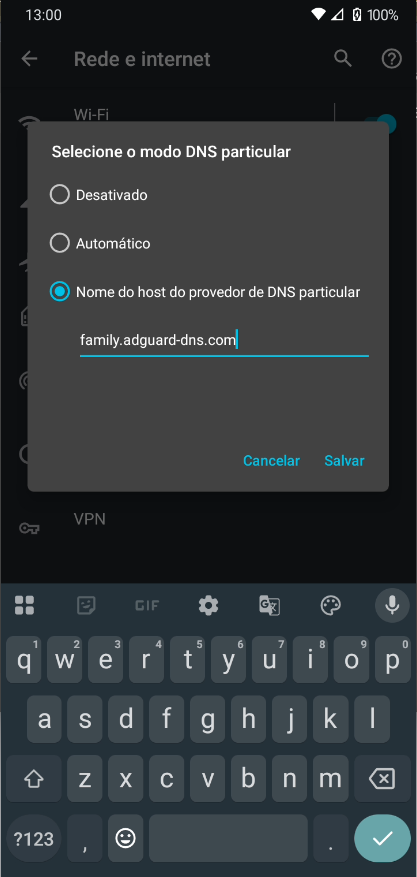
\includegraphics[align=c, width=\textwidth]{../../assets/screenshots/print_dns.png}
    \captionof*{figure}{\footnotesize \textcolor{NordText!80}{DNS Privado}}
\end{minipage}

\newpage

% ================= PÁGINA 4: SEÇÃO 2 (ECONOMIA GLOBAL) =================
\large{\textbf{\textcolor{BraveOrange}{2. Ativar a Economia de Dados}}}
\normalsize

\passo{BraveOrange}{1}{Nas \textbf{Configurações}, utilize a \textbf{Barra de Pesquisa} no topo.}
\passo{BraveOrange}{2}{Pesquise por \textbf{Economia de dados} e acesse o menu.}
\passo{BraveOrange}{3}{Ative a opção \textbf{Usar Economia de dados}. Isso bloqueia o tráfego em lote de aplicativos inativos.}

\vspace{4mm}
\begin{minipage}[t]{0.48\textwidth}
    \centering
    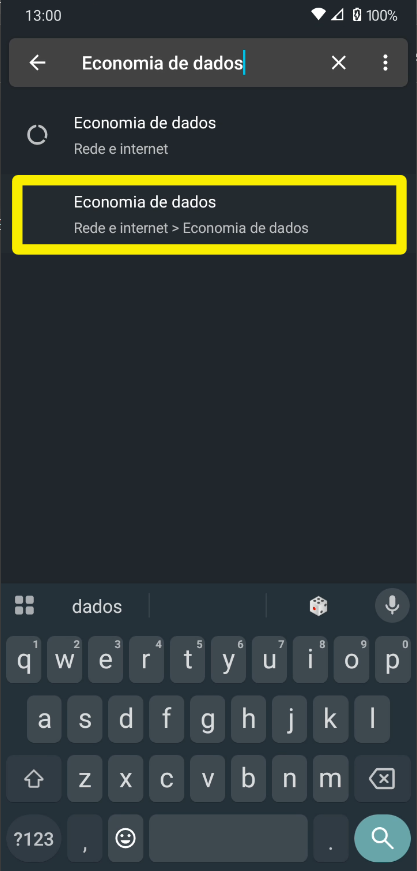
\includegraphics[align=c, width=\textwidth]{../../assets/screenshots/print_pesquisa.png}
    \captionof*{figure}{\footnotesize \textcolor{NordText!80}{Pesquisar}}
\end{minipage}
\hfill
\begin{minipage}[t]{0.48\textwidth}
    \centering
    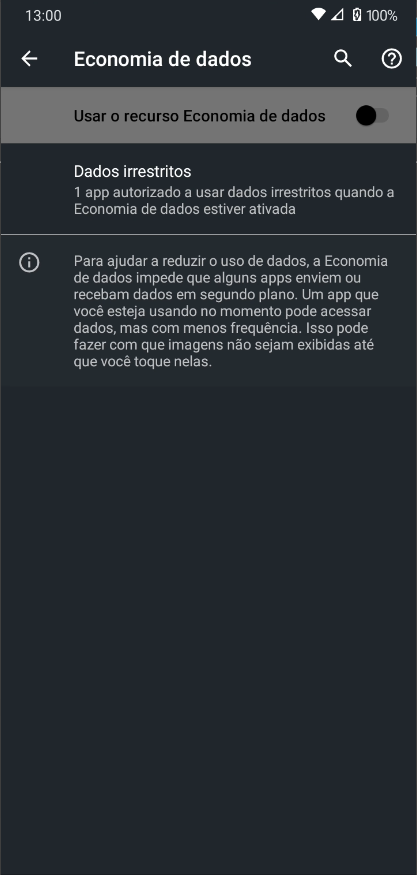
\includegraphics[align=c, width=\textwidth]{../../assets/screenshots/print_economia.png}
    \captionof*{figure}{\footnotesize \textcolor{NordText!80}{Ativar Recurso}}
\end{minipage}

\newpage

% ================= PÁGINA 5: SEÇÃO 3 (RESTRINGIR APPS - PARTE 1) =================
\large{\textbf{\textcolor{NordBlue}{3. Restringir Processos em 2º Plano}}}
\normalsize

\passo{NordBlue}{1}{Nas \textbf{Configurações}, acesse \textbf{Aplicativos} (ou Apps).}
\passo{NordBlue}{2}{Selecione aplicativos não essenciais que realizam sincronização constante (ex: redes sociais).}

\vspace{4mm}
\begin{minipage}[t]{0.48\textwidth}
    \centering
    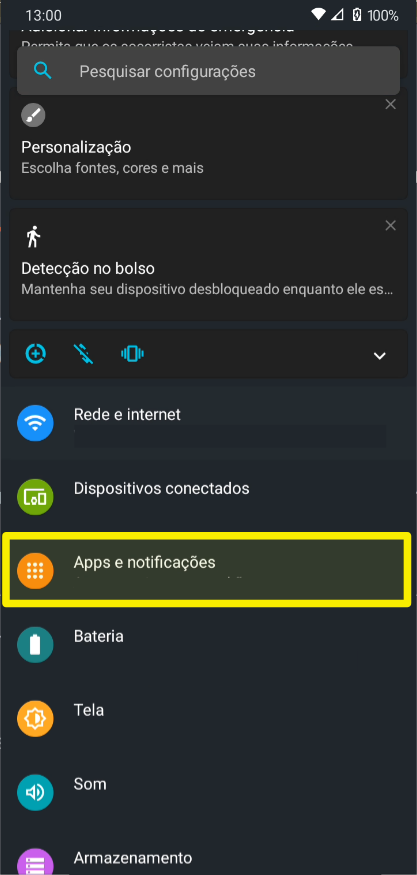
\includegraphics[align=c, width=\textwidth]{../../assets/screenshots/print_app1.png}
    \captionof*{figure}{\footnotesize \textcolor{NordText!80}{Lista de Apps}}
\end{minipage}
\hfill
\begin{minipage}[t]{0.48\textwidth}
    \centering
    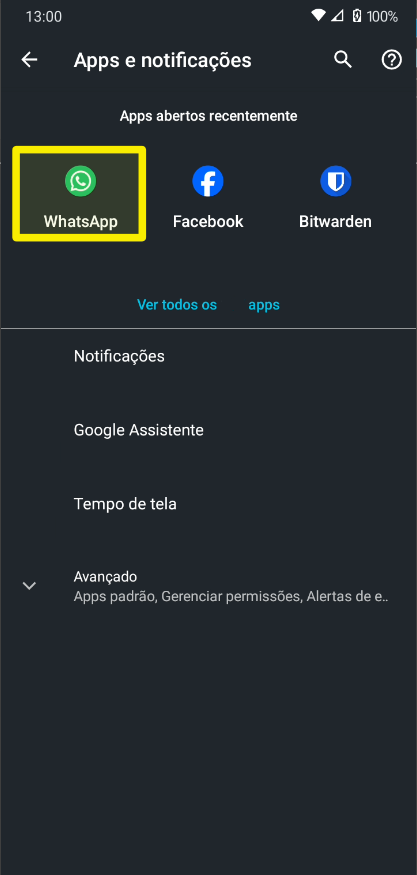
\includegraphics[align=c, width=\textwidth]{../../assets/screenshots/print_app2.png}
    \captionof*{figure}{\footnotesize \textcolor{NordText!80}{Selecionar App}}
\end{minipage}

\newpage

% ================= PÁGINA 6: SEÇÃO 3 (RESTRINGIR APPS - PARTE 2) =================
\large{\textbf{\textcolor{NordBlue}{3. Restringir Processos (Continuação)}}}
\normalsize

\passo{NordBlue}{3}{Toque em \textbf{Dados móveis e Wi-Fi} e desative \textbf{Dados em segundo plano}.}
\passo{NordBlue}{4}{Em seguida, vá em \textbf{Bateria} e mude para \textbf{Restrito}. Isso impede que o app acorde o processador quando ocioso.}

\vspace{4mm}
\begin{minipage}[t]{0.48\textwidth}
    \centering
    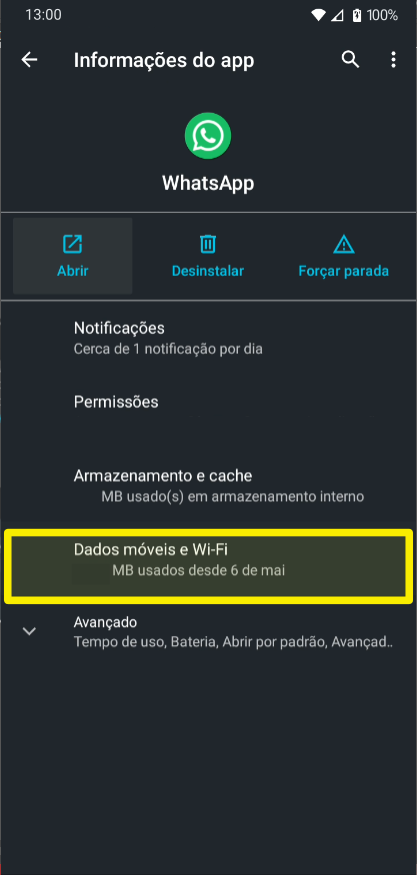
\includegraphics[align=c, width=\textwidth]{../../assets/screenshots/print_app3.png}
    \captionof*{figure}{\footnotesize \textcolor{NordText!80}{Dados do App}}
\end{minipage}
\hfill
\begin{minipage}[t]{0.48\textwidth}
    \centering
    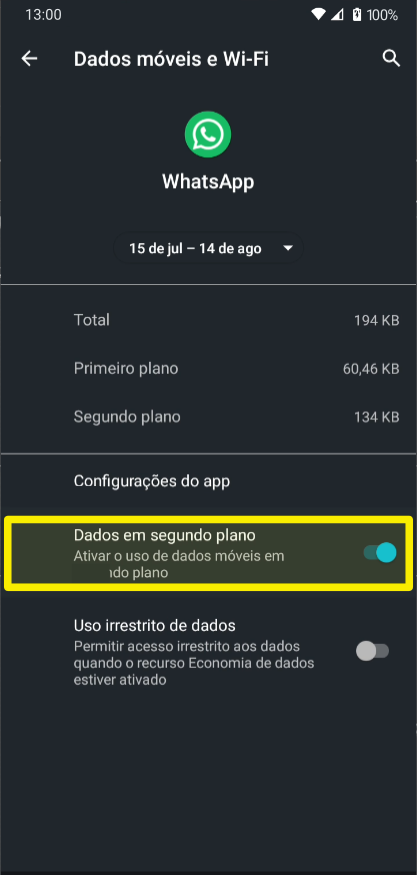
\includegraphics[align=c, width=\textwidth]{../../assets/screenshots/print_app4.png}
    \captionof*{figure}{\footnotesize \textcolor{NordText!80}{Bateria Restrita}}
\end{minipage}

\newpage

% ================= PÁGINA 7: SEÇÃO 4 (DOWNLOAD AUTOMÁTICO WHATSAPP) =================
\large{\textbf{\textcolor{NordPurple}{4. Desativar Mídia Automática}}}
\normalsize

\passo{NordPurple}{1}{No WhatsApp, abra \textbf{Configurações} > \textbf{Armazenamento e dados}.}
\passo{NordPurple}{2}{Em "Download automático de mídia", abra \textbf{Ao utilizar dados móveis}.}
\passo{NordPurple}{3}{Desmarque todas as mídias (\textbf{Fotos, Áudio, Vídeo, Documentos}) e confirme em \textbf{OK}.}

\vspace{4mm}
\begin{minipage}[t]{0.48\textwidth}
    \centering
    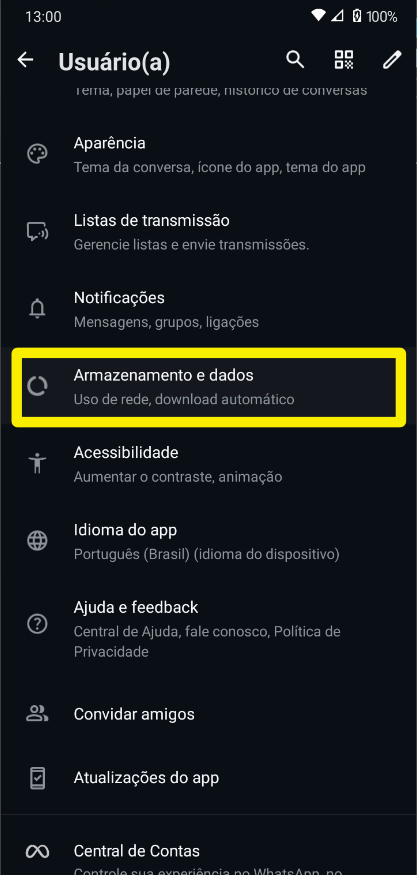
\includegraphics[align=c, width=\textwidth]{../../assets/screenshots/print_wpp2.png}
    \captionof*{figure}{\footnotesize \textcolor{NordText!80}{Armazenamento}}
\end{minipage}
\hfill
\begin{minipage}[t]{0.48\textwidth}
    \centering
    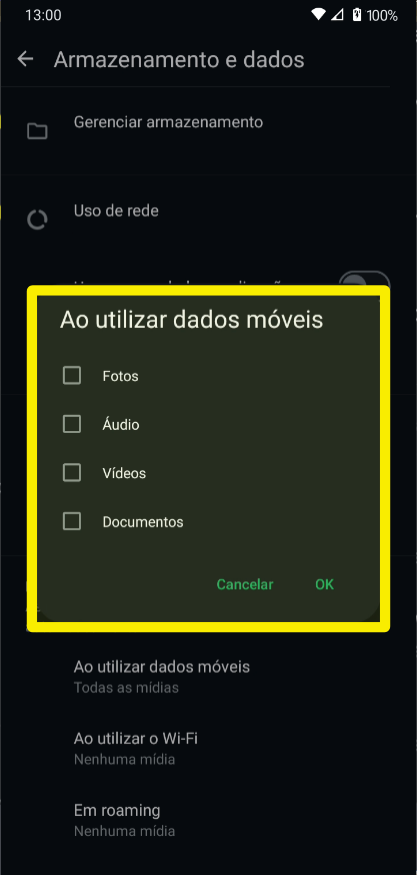
\includegraphics[align=c, width=\textwidth]{../../assets/screenshots/print_wpp4.png}
    \captionof*{figure}{\footnotesize \textcolor{NordText!80}{Desmarcar Tudo}}
\end{minipage}

\newpage

% ================= PÁGINA 8: SEÇÃO 5 (SAÚDE DA BATERIA) =================
\large{\textbf{\textcolor{AccentYellow}{5. Preservação de Ciclos de Carga}}}
\normalsize

\passo{AccentYellow}{1}{Nas \textbf{Configurações}, acesse o menu \textbf{Bateria}.}
\passo{AccentYellow}{2}{Toque em \textbf{Proteção da bateria} (ou Carregamento Otimizado).}
\passo{AccentYellow}{3}{Ative o limite de \textbf{80\%}. Isso reduz o estresse térmico e de voltagem nas células de lítio, prolongando a vida útil física do aparelho.}

\vspace{4mm}
\begin{minipage}[t]{0.48\textwidth}
    \centering
    
\includegraphics[align=c, width=\textwidth]{../../assets/screenshots/print_bateria1.png}
    \captionof*{figure}{\footnotesize \textcolor{NordText!80}{Menu Bateria}}
\end{minipage}
\hfill
\begin{minipage}[t]{0.48\textwidth}
    \centering
    
\includegraphics[align=c, width=\textwidth]{../../assets/screenshots/print_bateria2.png}
    \captionof*{figure}{\footnotesize \textcolor{NordText!80}{Proteção 80\%}}
\end{minipage}

\vfill
\begin{center}
    \tiny{\textcolor{NordText!50}{Projeto Multidisciplinar em Ciência da Computação | UFBRA}}
\end{center}

\newpage

% ================= PÁGINA 9: CONCLUSÃO E TELEMETRIA =================
\begin{center}
    \Large{\textbf{\textcolor{AdguardGreen}{\faCheckCircle \ Dispositivo Otimizado!}}}
    \vspace{2mm}
    \hrule
\end{center}

\vspace{3mm}

{\small \textbf{Impacto Ecológico Direto:} Com essas etapas, você reduziu a sobrecarga do modem 4G/5G, estancou requisições ocultas a servidores remotos e protegeu a bateria contra degradação prematura. Compartilhe esta prática na sua comunidade escolar!}

\vspace{4mm}

\begin{tcolorbox}[colback=NordBg, coltext=NordText, colframe=AccentYellow, boxrule=1pt, arc=4pt, left=2mm, right=2mm]
    \centering
    \textbf{\textcolor{AccentYellow}{Validação da Aplicação}}\\[2mm]
    {\scriptsize Escaneie o QR Code ou toque no link abaixo para registrar anonimamente a conclusão das configurações. Este endpoint alimenta a telemetria aberta do projeto.}\\[3mm]
    
    
\includegraphics[width=2.5cm]{../../assets/qr_cuttly_edu_ok.png}\\[2mm]
    
    \begin{center}
        \href{https://cutt.ly/edu-ok}{\textbf{\textcolor{AdguardGreen}{\faLink \ CLIQUE AQUI PARA REGISTRAR O SEU OK!}}}
    \end{center}
\end{tcolorbox}

\vfill

\begin{center}
    \scriptsize
    {\small Ciência da Computação — UFBRA}\\[2mm]
    \href{https://github.com/naygno/green-computing-edu}{\textcolor{NordText!80}{\faGithub \ github.com/naygno/green-computing-edu}}
\end{center}

\end{document}